\documentclass{article}

\usepackage{graphicx}
\usepackage{natbib}
\usepackage{amsmath}
\usepackage{amssymb}
\usepackage{enumerate}
\usepackage{setspace}
\usepackage{dsfont}
\usepackage{multirow}
\usepackage{chngpage}

\pagestyle{myheadings}
\markright{}

\renewcommand\footnotemark{}

\bibpunct{(}{)}{,}{a}{,}{,}

\onehalfspacing

\hyphenation{multi-currency}
\hyphenation{sub-period}

\title{Managing currency risk: An application of copula-based multivariate
dynamic models}
\author{Alexandre Beaulne, HEC Montr\'eal \and Bruno R\'emillard, HEC Montr\'eal
\and Pierre Laroche, National Bank of Canada}

\begin{document}

\abovedisplayskip=0.5cm
\abovedisplayshortskip=0.4cm
\belowdisplayskip=0.5cm
\belowdisplayshortskip=0.4cm

\maketitle\thispagestyle{empty}

\begin{abstract}
\addcontentsline{toc}{section}{Abstract}
In order to access foreign markets, global investors often need to post collateral in
currencies that are different from their benchmark currency, resulting in undesired
foreign exchange risk. Investors might therefore be tempted to strictly post the
minimum margins required, however doing so maximizes the probability of margin
calls and their associated operational risk and cost. This article finds the posted margins
that represent the best equilibrium between foreign exchange risk and probability
of a margin call. In order to do so, a robust dynamic model of the asset prices and exchange
rates dynamics is proposed, and an optimization problem seeking the optimal equilibrium is
solved. The proposed model overperformed both a naive and a Gaussian alternative
model on a dataset of five futures contracts in four different currencies over a 
period of six years for the metrics of interest.
\end{abstract}


\renewcommand{\thefootnote}{}
\footnotetext{\hspace*{-.51cm}AMS 2010 subject classification: Primary: 91G10, 91G70\\
Key words and phrases: copula-based multivariate dynamic models, foreign exchange risk,
multidimensional constrained optimization, collateral management}

\section{Introduction}
With the globalization of financial markets, investors have access to a larger
investment universe giving them the opportunity to better diversify their
portfolio. A subclass of financial transactions (short selling and entering
into derivative contracts for example) requires the posting of margins, that is,
the deposit of collateral to attenuate the credit risk for the counterparty. If
such a transaction is performed in a foreign market, the required collateral
will most likely be in a currency different from the portfolio's benchmark
currency, creating foreign exchange risk for the global investor. This investor
might therefore want to maintain the posted collateral to the strict minimum.
This policy will however maximize the probability that the counterparty, either
the investor's broker or exchange, will require the posting of additional
collateral following an adverse price change, so-called a margin call.

Margin calls sometimes result in undesired operational costs for investors, they
are therefore to be avoided if possible. Not only counterparties may impose
penalties on margin calls, but the regulatory framework agreed upon by members
of the Basel Committee on Banking Supervision in the Basel III accords impose
tougher capital buffers and liquidity coverage on derivatives transactions
\citep{basel1,basel2}.

The purpose of this work is to use recent developments in the field of
econometrics to come up with a  rigorous solution to the problem of
multicurrency collateral management. In addition, the methodology proposed here
can be extended to many financial and risk management applications where an
optimization problem needs to be constrained by practical considerations
(transaction costs for example). 

The quest to a better understanding and forecasting of financial time series
resulted in a constant increase in the level of sophistication of econometrics
models. For univariate series, the canonical Brownian process
\citep{brown1828, bachelier1900, merton69} has often been substituted with more
recent models capturing empirical properties of the financial time series such
as heteroskedasticity and leptokurticity (fat tails). The most popular of these
models are AutoRegressive Conditionnal  Heteroskedasticity (ARCH) \citep{engle82}
and its extension the generalized ARCH (GARCH) \citep{bollerslev86}. In these
models, the variance, and hence the volatility, of the time series for a given
period is a direct function of the variance in the previous period, thus
accounting for volatility clustering. Furthermore, the processes generate data
with fatter tails than the normal density. Thanks to its parsimonious notation
(see equations \eqref{drift} and \eqref{volatility} in Section~\ref{modelling}),
GARCH has become the most popular ARCH model in practice, including this work.

Proper financial modeling requires the consideration of dependence
between time series. For this reason the development of multivariate models
quickly followed the one of univariate models. It is now widely accepted
\citep{cont01, yue12} that robust risk management requires the inclusion of
higher-order moments and co-moments in the time series of financial assets.
Not only do univariate distributions capturing higher moments need to be picked
to model single financial time series, but a model of dependence between the
different time series allowing for higher co-moments is primordial. Indeed,
traditional linear correlation between the returns of financial assets fails
to capture the ``correlation breakdown'' or ``assets boom alone but bust
together'' asymmetry observed in the markets. Models have been proposed to
extend the ARCH-type framework described in the  previous paragraphs to
multivariate settings. They all face the challenge of balancing sophistication
with parsimony, of being flexible enough to capture co-moment dynamics while
avoiding the curse of dimensionality. For a comprehensive survey of
multivariate GARCH models, refer to \cite{silvennoinen08} or \cite{laurent06}.

A promising family of multivariate models combines the tractability of univariate
processes with the power of copulas to capture the dependence between the marginal
process in a robust manner. A copula, in combination with the univariate marginal
distributions,  is sufficient to fully specify a multivariate distribution
function, as proven by \cite{sklar59}. The copula $C$ underlying the random
variables $X_1$, $X_2$, $\ldots$, $X_D$ is the joint cumulative distribution
function of the transformed variables $F_1(x_1), F_2(x_2), \ldots,  F_D(x_D)$,
where $F_i(x)=\mathbb{P}[X_i \leq x]$ are the marginal cumulative distribution
functions, and
\begin{displaymath}
C(u_1, \ u_2, \ \ldots \ , u_D)=\mathbb{P}[F_1(X_1) \leq u_1, \
F_2(X_2) \leq u_2, \ \ldots \ , F_D(X_D) \leq u_D].
\end{displaymath}
This work owes much to the findings of Chen Xiaohong and Fan Yanqin
\citep{chenfan06}, Andrew Patton \citep{patton00,patton06} and Bruno
R\'emillard \citep{Remillard11}. The basis of these articles is that
the dependence between the error terms of multivariate time series
is described not in term of traditional correlation but by a given
copula.

Unfortunately, copulas have often been used prior to the existence of
proper goodness-of-fit tests, that is, without properly testing whether
the data being modeled belongs to the chosen copula or not in a
statistically significant manner. One of the first instance of copulas
goodness-of-fit test for multivariate time series  can be found in
\cite{chenfan06}, however this test can only rank the appropriateness
of different copulas relative to each other, not in a statistically
absolute sense. Fortunately, \cite{genestetal09} and \cite{Remillard11}
applied the parametric bootstrapping technique to copulas allowing one
to do so in an intuitive, powerful manner. Its use with copulas evolved
naturally from previous applications to univariate and multivariate
distributions. The application of this test prevents the use of a copula
where inappropriate.

The tools developed in this work can also be applied to related problems:
balancing tracking error and transaction costs (see \cite{chanramkumar11}),
foreign currency risk and hedging costs (see \cite{campbell2010}), sales
and marketing costs, etc. In the case of balancing foreign exchange risk
on posted collateral and the costs associated to margin calls, global
investors have historically used heuristics or more sophisticated policies
to mitigate the two inconveniences. For literature on the subject, one
can refer to \cite{MillerOrr, higson10} for solutions to the similar
problem of optimal inventory management, to \cite{cotter01,lam04,kao10,longin99}
for solutions to the problem of setting the margins requirements
by a central counterparties (e.g. clearing houses) and to
\cite{fujii2010} for an example where the market participant has
the choice of collateral currency.

The remainder of this article is organized as follows. Section~\ref{modelling}
exhibits the framework used to model the dynamics of the asset prices and
exchange rates. Section~\ref{optimisation} overviews the optimization problem at
hand. Section~\ref{backtesting} presents the results of a backtest of the
proposed solution performed on a real data set. Section~\ref{conclusion}
concludes and proposes avenues of future research.


\section{Copula-based multivariate dynamic models}
\label{modelling}
In order to develop a cash management strategy which strikes an optimal balance
between the opposing goals of minimizing foreign exchange risk and minimizing
the cost associated with margin calls, it is first necessary to choose a model of underlying asset prices
and exchange rates movements. It is now widely accepted that proper modeling
is robust to volatility clustering and excess kurtosis. That is, the volatility in
financial time series is not constant across time but periods of relatively high volatility
tend to cluster together. Furthermore, the probability of extreme events in the joint
distributions of multivariate financial time series innovations is higher than predicted
under a Gaussian model. The latter phenomenon is also known as ``fat tails''.
Refer to \cite{pagan96, cont01}
for evidence of stylized facts of financial time series and more precisely to
\cite{casper94, guillaume97} for evidence of such facts in exchange rate returns.

We propose the use of a dynamic multivariate discrete stochastic volatility model
with a copula-based dependence structure. This model has been successfully applied
to exchange rate returns in the literature \citep{chenfan06,Remillard11,patton06}. The
multivariate time series $\mathbf{X}_t$, $t\geq 1$ has $D$ dimensions and is given by
\begin{equation}
\label{dynmodel}
    X_{i,t}=\mu_t(\boldsymbol\theta_i)+h_t(\boldsymbol\theta_i)^{1/2} \
    \epsilon_{i,t},
\end{equation}
where $i=1,\ldots,D$
and innovations $\epsilon_{1,t},\ldots,\epsilon_{D,t}$ are \emph{i.i.d.} with
copula distribution function $C$.

We know from Sklar theorem \citep{sklar59} that, given that $K$ is continuous, there
exists a unique copula $C$ such that
\begin{equation}
\label{sklar}
     K(x_1,\ldots,x_D)=C_{\boldsymbol\theta}(F_1(x_1),\ldots,F_D(x_D)),
\end{equation}
where the $F_i$ are the cumulative distribution
functions of the marginal distributions $X_i$ and $C_{\boldsymbol\theta}$ is the copula
function with parameter(s) $\boldsymbol\theta$.

An interesting property of copulas is that the dependence between the variables is
encapsulated in the copula function and is independent of the marginal distribution
functions chosen.

We model the marginal distributions of the financial time series
with AR(k)-GARCH(p,q) models \citep{bollerslev86}. We chose this
model because we believe it offers the best equilibrium between
sophistication and parsimony. Their formulation is given by
\begin{equation}
\label{drift}
    \mu_t(\boldsymbol\theta_i)=\kappa_{\mu,i}+ \sum_{j=1}^k \gamma_{i,j} \
    x_{i,t-j},
\end{equation}
and
\begin{equation}
\label{volatility}
    h_t(\boldsymbol\theta_i)=\kappa_{h,i} + \sum_{j=1}^q \alpha_{i,j} \ \epsilon_{i,t-j}^2 +  \sum_{j=1}^p \beta_{i,j} \
    h_{t-j}(\boldsymbol\theta_i).
\end{equation}

We tested the goodness-of-fit of common elliptical (Gaussian and
Student) and Archimedean (Clayton, Frank, Gumbel)  copulas on the
standardized residuals of the AR-GARCH margins processes emerging
from the dataset described in section \ref{dataset}. Their
distributions are given below, and the recipe of the parametric
bootstrapping goodness-of-fit tests is given in Appendix \ref{GOF}.

The Gaussian copula with dependence parameter matrix $\Sigma$ is given by
\begin{equation}
\label{gaussiancopuladist}
C_{\Sigma}(\mathbf{u})=\Phi_{\Sigma}\left(\Phi^{-1}(u_1), \ \ldots
\, \Phi^{-1}(u_D)\right),
\end{equation}
where $\Phi^{-1}(\cdot)$ is the inverse cumulative distribution function of a standard normal, $\Phi_{\Sigma}(\cdot)$ is the joint
cumulative distribution function of a multivariate normal distribution with zero means and covariance matrix $\Sigma$. Its density is given by
\begin{displaymath}
c_{\Sigma}(\mathbf{u})=\left| \Sigma \right|^{-\frac{1}{2}} \
\exp\left(-\frac{1}{2}  \left(\begin{array}{c} \Phi^{-1}(u_1)\\
\vdots \\  \Phi^{-1}(u_D) \end{array}  \right)^T
(\Sigma^{-1}-\mathbf{I}) \left(\begin{array}{c} \Phi^{-1}(u_1)\\
\vdots \\  \Phi^{-1}(u_D) \end{array}  \right)\right).
\end{displaymath}

The \emph{D}-dimensional Student copula distribution as given by \citep{mcneil05}:
\begin{equation}
\label{tcopuladist} C_{\Sigma,\nu}(\mathbf{u}) =
\int_{-\infty}^{t_{\nu}^{-1}(u_1)}  \ldots
\int_{-\infty}^{t_{\nu}^{-1}(u_D)} \frac{\Gamma\left(
\frac{\nu+D}{2}\right)}{\Gamma \left( \frac{\nu}{2} \right)
\sqrt{(\pi \nu)^D |\Sigma|}} \left( 1+\frac{\mathbf{x}' \Sigma^{-1}
\mathbf{x}}{\nu}\right)^{-\frac{\nu+D}{2}} d\mathbf{x},
\end{equation}
where
$t_{\nu}^{-1}()$ is the quantile function of a standard univariate Student distribution with $\nu$
degrees of freedom. Its density can be derived to be
\begin{equation}
\label{tcopuladens}
c_{\Sigma,\nu}(\mathbf{u})=\frac{f_{\Sigma,\nu}(t_{\nu}^{-1}(u_1),\ldots,t_{\nu}^{-1}(u_D))}{\prod_{i=1}^D
f_{\nu}(t_{\nu}^{-1}(u_i))},
\end{equation}
where $f_{\Sigma,\nu}$ is the joint density of a D-dimensional random vector from a multivariate
Student distribution with $\nu$ degrees of freedom and covariance matrix $\Sigma$ and
$f_{\nu}$ is the density of a univariate Student distribution with $\nu$ degrees of freedom.
 This copula not only captures excess kurtosis but was also shown to accurately model
the dependence between financial time series in recent literature \citep{chenfan06,fisher09}.

Archimedean copulas are characterized by a single dependence parameter and the following representation:
\begin{displaymath}
C(u_1, \ u_2, \ \ldots \ ,
u_D)=\psi(\psi^{-1}(u_1)+\ldots+\psi^{-1}(u_D)),
\end{displaymath}
where $\psi(\cdot)$ is the \emph{generator} of the copula. The
generators for the three Archimedean copulas tested in the applied
section of this thesis are displayed in table \ref{archi}.
\begin{table}[htb]
    \centering
    \begin{footnotesize}
    \begin{tabular}{c c c c}
    \textbf{Family}&\textbf{Generator} $\boldsymbol\psi\mathbf{(t)}$&\textbf{Parameter}&$\mathbf{G}$\textbf{-distribution}\\
    Clayton&$(1+t)^{-1/\theta}$&$0 < \theta < \infty$&Gamma$(1/\theta,1)$\\
    Frank&$-\frac{1}{\theta}\log(1-(1-e^{-\theta}) e^{-t})$&$0 < \theta < \infty$&Log series with $\alpha=(1-e^{-\theta})$\\
    Gumbel&$\exp(-t^{1/\theta})$&$1 \leq \theta < \infty$&Stable$(1/\theta,1,(\cos(\pi/(2\theta)))^{\theta},0)$\\
    \end{tabular}
    \end{footnotesize}
    \caption[Generators of selected Archimedean copulas]{Generators of selected Archimedean copulas. G-distribution refers to the
distribution that has as Laplace transform the generator $\psi(\cdot)$.}
    \label{archi}
\end{table}


The parameters of the marginal processes and dependence copula can
be estimated with the maximum likelihood estimation (MLE) method. An
alternative two-stage estimation method for the Student copula
is proposed by \cite{mcneil05b}.

\cite{chenfan06} showed the important result that applying the copula dependence structure
from equation (\ref{sklar}) to the innovations $\epsilon_{i,t}$ from equation (\ref{dynmodel}) rather
than to the realizations $X_{i,t}$ yields the same results
in terms of estimation of the parameters of the copula. \cite{Remillard11} showed that
the empirical copula and most dependence measures are unaffected as well.



\section{Constrained optimization}
\label{optimisation}
One difficulty in the problem at hand is to find a way to balance foreign exchange risk on
one hand and the costs associated to margin calls on the other. This exercise proves difficult
given that these two forces have different units. We posited that the costs associated to
margin calls are an increasing function of their frequency, and chose to minimize the foreign exchange
risk on the posted collateral conditionally to an arbitrary upper bound on the probability
of a margin call. \cite{chanramkumar11} offers an elegant framework
to a problem similar in nature to ours. Their goal is to balance trading costs associated
with the rebalancing of a given portfolio and tracking error. Their solution is to
minimize the trading costs subject to an imposed upper ceiling on the forecasted
tracking error. Our objective function described below is inspired from this approach.

We formulate the issue at hand as a one-period constrained optimization problem.
The first step consists in choosing a risk measure to assess the foreign exchange
risk. This work uses the expected tracking error (ETE), the Value-at-Risk (VaR) and
the Tail Conditional Expectation (TCE). The method consists in finding the cash
balances that minimize the (foreign exchange) risk measure subject to an arbitrary
tolerance for the probability of a margin call. A mathematical formulation of the
optimization objective is
\begin{equation}
\label{riskmeasure} \min_{\lambda_{1,t}, \ldots, \lambda_{D,t}}
R^{\alpha}\left( \sum_{i=1}^D \left( \lambda_{i,t} -
\lambda_{i,t}^{\ast} \right) \cdot Y_{i,t+1} \right),
\end{equation}
where
\begin{equation}
\label{riskmeasure2}
R^{\alpha}(X) = \left\{ \begin{array}{cl}
              \mathbb{E}\left[ \left| X\right| \right] & \mbox{ for expected tracking error}, \\
              -\mathbb{Q}_{\alpha}(X) & \mbox{ for Value-at-Risk}, \\
              -\mathbb{E}[X|X\leq \mathbb{Q}_{\alpha}(X)] & \mbox{ for Tail Conditional Expectation}. \\
       \end{array} \right.
\end{equation}
where $\mathbb{Q}_{\alpha}(X)$, $\alpha \ \in \ [0,1]$ is a  quantile of $X$
such that $P(X\leq\mathbb{Q}_{\alpha}(X))=\alpha$. In words,
equation~(\ref{riskmeasure}) finds the collateral in each
currency $\lambda_{1,t}, \ldots, \lambda_{D,t}$  above the minimum
margins requirements imposed by the counterparty
$\lambda_{1,t}^{\ast}$, $\ldots$, $\lambda_{D,t}^{\ast}$ that
minimizes one of the risk measures $R^{\alpha}(\cdot)$ described in
equation~(\ref{riskmeasure2}) against the changes in the exchange
rates $Y_{1,t+1}$, $\ldots$, $Y_{D,t+1}$.
The first constraint of the optimization is
\begin{displaymath}
\lambda_{i,t}^{\ast}\leq\lambda_{i,t}\leq\infty,\ i=1,\ldots,D,
\end{displaymath}
that is, each posted collateral $\lambda_{i,t}$ must be between the
minimum margin requirement $\lambda_{i,t}^{\ast}$ and infinity.  The
second constraint of the optimization is
\begin{displaymath}
%\label{probmargincall}
\mathbb{P} \left( \left( \prod_{i=1}^D \mathds{1}\left(
\lambda_{i,t} + \mbox{PnL}_{i,t+1}\geq
\lambda_{i,t}^{\ast}\right)\right)=0 \right) \leq P_{\mbox{tol}},
\end{displaymath}
where
\begin{displaymath}
%\label{pnl}
\mbox{PnL}_{i,t+1}=\sum_{j=1}^{n_{i,t}} {}_i\omega_{j,t} \cdot {}_i
W_{j,t+1}.
\end{displaymath}
Here, $P_{\mbox{tol}}$ is an arbitrary tolerance for the probability
of a margin call,  $n_{i,t}$ is the number of different assets of
the $i^{th}$ currency held,  ${}_i\omega_{j,t}$ is the number of the
$j^{th}$ asset of the  $i^{th}$ currency held and ${}_i W_{j,t+1}$
is the change in the $j^{th}$ asset of the $i^{th}$ currency between
time $t$ and $t+1$. To make things clear, the only random variables
in the model are the $Y_{i,t}$ and the ${}_i W_{j,t+1}$.
Furthermore, these random variables are not independent of each
other. That is, the spot exchange rates are not independent of the
futures contracts prices and vice versa.

The proposed methodology for the optimization is as follow: First,
univariate process are fitted to each time-series of log returns of
exchange rates and future prices. This step often involves the
calibration of parameters with the maximum likelihood estimation
method. Second, goodness-of-fit tests of the selected model are
performed on each time-series. If the test result is negative for a
given time-series of log returns, then another univariate model is
chosen for that specific time-series and the process is started anew
from the first step. Again, different time-series can have different
univariate models. Third, a parametric multivariate copula is fitted
to the normalized ranks of the standardized residuals obtained in
the first step. Fourth, a goodness-of-fit test as put forward in
Appendix~\ref{GOF} is performed on the copula-based dynamic model
with respect to the sample of time-series. If the test result is
negative, another copula is chosen and the process is restarted from
the third step. At this point, we know that the model is appropriate
for the data (at least in the statistical sense of the term). Here
is where Monte Carlo methods come into play. Fifth, a large number
$N$ of $D$-dimensional $U[0,1]$ realizations is drawn from the
parametric copula, were $D$ is the number of time-series modeled.
Most modern statistical software packages provide tools to perform
this step for elliptical copulas. One can refer to \cite{marshallolkin88}
and to \cite{melchiori06} for Archimedean copula random variable
gerneration. Sixth, the simulated standardized residuals
of each univariate process are obtained by entering the uniform
drawings from the previous step into their respective inverse
cumulative distribution function. Seventh, the simulated
realizations of the log returns are obtained by combining of the
random standardized residuals and the computed deterministic part of
each univariate process. The final step consists in using
constrained numerical optimization to find the values of the control
variables that optimize the objective function while satisfying the
constraint function. For us, the control variables are the amount of
collateral held in each currency, the objective function is the risk
measure (tracking error, Var and TCE) and the constraint function is
the probability of a margin call. Notice that both the objective and
constraint are functions of the control variables (the amount of
collateral held in each foreign currency) and the
realizations from the Monte Carlo simulation (the log returns of
exchange rates and future prices). The objective and constraint
functions being nonlinear, we obtained the best results using the
interior point optimization method, closely followed by the active
set algorithm.


\section{Backtesting}
\label{backtesting}
\subsection{Dataset}
\label{dataset} In order to demonstrate the validity of the model
proposed in the previous sections, we compare its performance over a
data set against alternative strategies described in
Section~\ref{altstrats}. The data set consists of daily holdings of
five futures contracts denominated in non-USD currencies from
November 2003 to December 2012, for a total of 2115 observations.
Figure~\ref{prices} exhibits the future contracts prices and the
number of each contract held at any moment. These holdings are
exogeneous to our control; our aim is to find the optimal cash
margins given certain holdings of contracts denominated in foreign
currencies.
\begin{figure}[htbp]
    \centerline{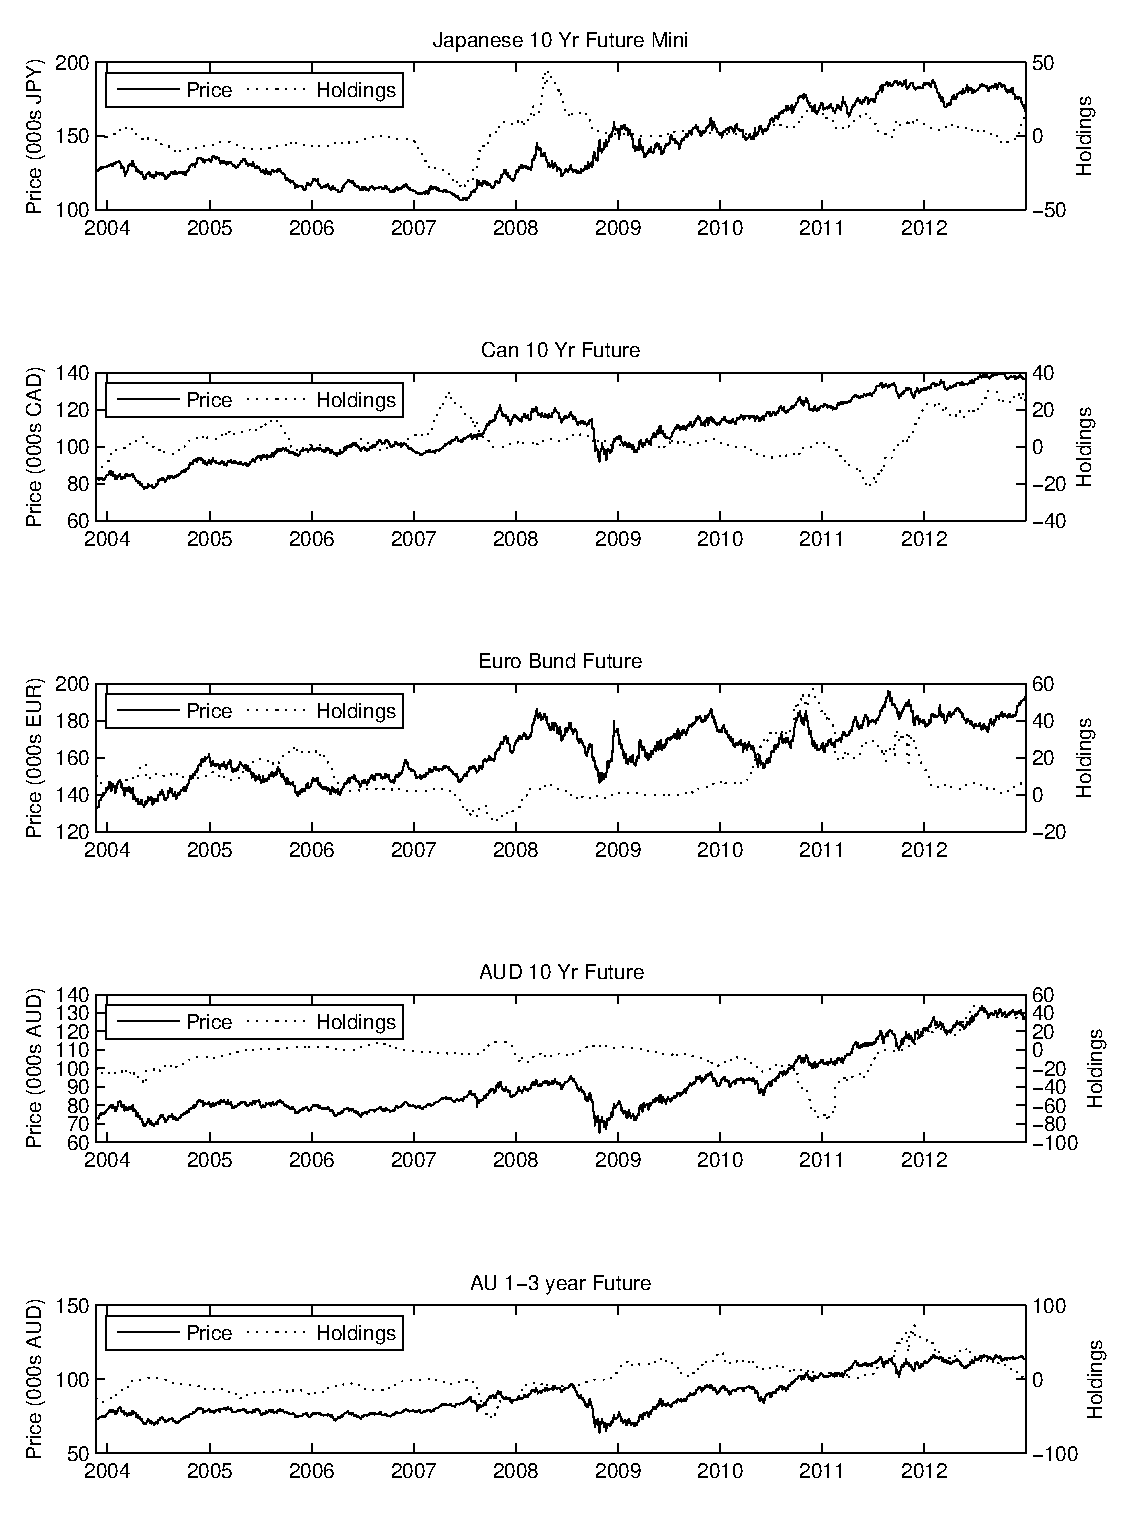
\includegraphics[scale=0.8]{contractsprices.eps}}
    \caption{Futures contracts prices and holdings}
\label{prices}
\end{figure}

A graphical test proposed by \cite{Gnanadesikan77} to test joint normality
was run on the data. If $\mathbf{X}=X_1, \ \ldots \ ,X_d$ is from a multivariate
Gaussian distribution, then
\begin{displaymath}
(\mathbf{X}_i-\bar{\mathbf{X}})' \ \Sigma \ (\mathbf{X}_i-\bar{\mathbf{X}}), \ i=1, \ \ldots \ ,N
\end{displaymath}
where $\Sigma$ is the covariance matrix of $\mathbf{X}$ have a $\chi^2_d$-distribution.
A QQ plot can then be used as a quick, ``litmus'' test of joint normality, as seen in
Figure~(\ref{mvQQplot}). Evidently joint normality has to be rejected.
\begin{figure}[htbp]
  \centerline{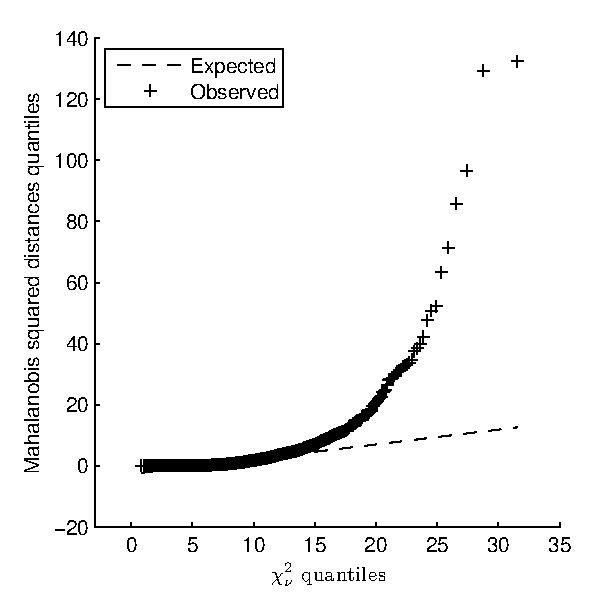
\includegraphics[scale=1]{mvQQplot.eps}}
   \caption{Graphical test of joint normality - QQ plot}
   \label{mvQQplot}
\end{figure}



\subsection{Alternative strategies}
\label{altstrats}
In order to access the validity of our model, we backtested it on
the dataset presented in the previous section. We also backtested
two other strategies on the same dataset to contrast their
performances.

The first, ``naive'' strategy simply consists in keeping twice the compulsory
collateral in the cash accounts at all times. That is, the collateral posted
in the accounts of the different currencies is brought back to twice the mandatory
minimum every day according to that day's movements in futures contracts prices
and holdings.

The second strategy consists in modeling the returns of the futures
contracts and exchange rates with a static multivariate normal
distribution as in the Markowitz framework. Doing so allows us to
gauge the accuracy added by factoring in stochastic volatility and
higher co-moments as done by the model proposed in
Section~\ref{modelling}.


\subsection{Calibration}
A buffer of 500 business days (approximately 2 years) is used at
the beginning of the sample to calibrate the marginal processes
and the dependence copula
parameters. The
means and covariance matrix for the static multivariate strategy
is also computed with this buffer. Both models are recalibrated
every day using all data from the beginning of the sample (i.e.
with an extending window).

The tolerance for the probability of a margin call $P_{tol}$ was
arbitrarily set to 0.05, which was also the level chosen for the
quantile $\alpha$ of the VaR and TCE measures.

Once at the beginning and then every 250 business days, with an
extending window, the goodness-of-fit tests described in
Appendix~\ref{GOF} were performed on both the marginal processes and
the dependence copulas. The results of the goodness-of-fit tests for
the AR(1)-GARCH(1,1) with Gaussian residuals, AR(2)-GARCH(2,2) with
Gaussian residuals, AR(1)-GARCH(1,1) with Student residuals and
different dependence copulas are displayed in
tables~\ref{ar1garch11}, \ref{ar2garch22}, \ref{ar1garch11_t} and
\ref{copulas} respectively. Clearly, a combination of
AR(1)-GARCH(1,1) with Student residuals and the Student copula is
the only appropriate model from a statistical point of view for the
time-series at hand.
\begin{table}[p]
    \begin{adjustwidth}{-1in}{-1in}
    \centering
    \begin{scriptsize}
\begin{tabular}{lccccccc}
&\textbf{Feb06}&\textbf{Mar07}&\textbf{Apr08}&\textbf{Apr09}&\textbf{May10}&\textbf{Jun11}&\textbf{Jun12}\\\hline
\textbf{Japanese 10 Yr Future Mini}&0.04&0.09&0.00&0.00&0.00&0.00&0.00\\
\textbf{Can 10 Yr Future}&0.11&0.55&0.55&0.03&0.02&0.01&0.01\\
\textbf{Euro Bund Future}&0.00&0.00&0.01&0.00&0.00&0.00&0.00\\
\textbf{AUD 10 Yr Future}&0.00&0.00&0.00&0.00&0.00&0.00&0.00\\
\textbf{AU 1-3 year Future}&0.07&0.07&0.00&0.01&0.00&0.00&0.00\\
\textbf{AUD/USD}&0.44&0.13&0.00&0.00&0.00&0.00&0.00\\
\textbf{CAD/USD}&0.15&0.26&0.08&0.00&0.00&0.00&0.00\\
\textbf{EUR/USD}&0.00&0.01&0.00&0.00&0.00&0.00&0.00\\
\textbf{JPY/USD}&0.05&0.02&0.00&0.00&0.00&0.00&0.00\\
\end{tabular}
\end{scriptsize}

    \end{adjustwidth}
    \caption[GOF tests of AR(1)-GARCH(1,1) with Gaussian residuals]{\emph{p}-values from the goodness-of-fit tests of AR(1)-GARCH(1,1) with Gaussian residuals on the marginal processes. The number of bootstrapped samples is $N=100$.}
    \label{ar1garch11}
\end{table}
\begin{table}[p]
    \begin{adjustwidth}{-1in}{-1in}
    \centering
    \begin{scriptsize}
\begin{tabular}{lccccccc}
&\textbf{Feb06}&\textbf{Mar07}&\textbf{Apr08}&\textbf{Apr09}&\textbf{May10}&\textbf{Jun11}&\textbf{Jun12}\\\hline
\textbf{Japanese 10 Yr Future Mini}&0.06&0.10&0.02&0.00&0.00&0.00&0.00\\
\textbf{Can 10 Yr Future}&0.12&0.48&0.39&0.01&0.00&0.00&0.00\\
\textbf{Euro Bund Future}&0.00&0.00&0.00&0.00&0.00&0.00&0.00\\
\textbf{AUD 10 Yr Future}&0.01&0.00&0.00&0.00&0.00&0.00&0.00\\
\textbf{AU 1-3 year Future}&0.04&0.01&0.00&0.00&0.00&0.00&0.00\\
\textbf{AUD/USD}&0.33&0.09&0.00&0.00&0.00&0.00&0.00\\
\textbf{CAD/USD}&0.09&0.35&0.11&0.00&0.00&0.00&0.00\\
\textbf{EUR/USD}&0.01&0.00&0.00&0.00&0.00&0.00&0.00\\
\textbf{JPY/USD}&0.07&0.01&0.00&0.00&0.00&0.00&0.00\\
\end{tabular}
\end{scriptsize}

    \end{adjustwidth}
    \caption[GOF tests of AR(2)-GARCH(2,2) with Gaussian residuals]{\emph{p}-values from the goodness-of-fit tests of AR(2)-GARCH(2,2) with Gaussian residuals on the marginal processes. The number of bootstrapped samples is $N=100$}
    \label{ar2garch22}
\end{table}
\begin{table}[p]
    \begin{adjustwidth}{-1in}{-1in}
    \centering
    \begin{scriptsize}
\begin{tabular}{lccccccc}
&\textbf{Feb06}&\textbf{Mar07}&\textbf{Apr08}&\textbf{Apr09}&\textbf{May10}&\textbf{Jun11}&\textbf{Jun12}\\\hline
\textbf{Japanese 10 Yr Future Mini}&0.42&0.57&0.62&0.51&0.55&0.58&0.41\\
\textbf{Can 10 Yr Future}&0.55&0.70&0.80&0.72&0.81&0.80&0.88\\
\textbf{Euro Bund Future}&0.34&0.42&0.43&0.28&0.33&0.45&0.56\\
\textbf{AUD 10 Yr Future}&0.58&0.54&0.54&0.49&0.63&0.51&0.43\\
\textbf{AU 1-3 year Future}&0.56&0.70&0.59&0.45&0.60&0.45&0.60\\
\textbf{AUD/USD}&0.71&0.70&0.55&0.49&0.51&0.42&0.48\\
\textbf{CAD/USD}&0.46&0.55&0.50&0.46&0.56&0.61&0.71\\
\textbf{EUR/USD}&0.32&0.53&0.36&0.26&0.44&0.47&0.57\\
\textbf{JPY/USD}&0.56&0.57&0.49&0.51&0.49&0.50&0.47\\
\end{tabular}
\end{scriptsize}

    \end{adjustwidth}
    \caption[GOF tests of AR(1)-GARCH(1,1) with Student residuals]{\emph{p}-values from the goodness-of-fit tests of AR(1)-GARCH(1,1) with Student residuals on the marginal processes. The number of bootstrapped samples is $N=100$.}
    \label{ar1garch11_t}
\end{table}
\begin{table}[htb]
    \begin{adjustwidth}{-1in}{-1in}
    \centering
    \begin{scriptsize}
\begin{tabular}{lccccccc}
&\textbf{Feb06}&\textbf{Mar07}&\textbf{Apr08}&\textbf{Apr09}&\textbf{May10}&\textbf{Jun11}&\textbf{Jun12}\\\hline
\textbf{MV Gaussian}&0.00&0.00&0.00&0.00&0.00&0.00&0.00\\
\textbf{AR(1)-GARCH(1,1) \& Gaussian copula}&0.13&0.04&0.00&0.00&0.00&0.00&0.00\\
\textbf{AR(1)-GARCH(1,1) \& Student copula}&0.64&0.17&0.34&0.21&0.17&0.23&0.19\\
\textbf{AR(1)-GARCH(1,1) \& Clayton copula}&0.00&0.00&0.00&0.00&0.00&0.00&0.00\\
\textbf{AR(1)-GARCH(1,1) \& Frank copula}&0.00&0.00&0.00&0.00&0.00&0.00&0.00\\
\textbf{AR(1)-GARCH(1,1) \& Gumbel copula}&0.00&0.00&0.00&0.00&0.00&0.00&0.00\\
\end{tabular}
\end{scriptsize}

    \end{adjustwidth}
    \caption[GOF test of dependence copulas]{\emph{p}-values from the goodness-of-fit tests of copulas. The marginal processes were modeled with AR(1)-GARCH(1,1) with Student residuals. The number of bootstrapped samples is $N=100$.}
    \label{copulas}
\end{table}

\subsection{Results}

Tables~\ref{resultsETE_complete},~\ref{resultsVaR_complete}~and~\ref{resultsTCE_complete}
exhibit the results of the backtests
over the entire sample for the three risk measures of interest.
The copula-based multivariate dynamic approach always had the
lowest frequency of margin
calls, while maintaining similar risk measures realizations.
\begin{table}[p]
    \begin{adjustwidth}{-1in}{-1in}
    \centering
    \begin{small}\begin{tabular}{ l c c c }
&\textbf{Naive}&\textbf{MV Gaussian}&\textbf{AR-GARCH \& t copula}\\
\textbf{Avg. daily tracking error (\% collateral)}&0.52&0.52&0.52\\
\textbf{\# of margin calls (out of 1614 days)}&110&99&85\\
\textbf{Frequency of margin call}&0.07&0.06&0.05\\
\end{tabular}
\end{small}

    \end{adjustwidth}
    \caption[Results of the backtests - Minimized ETE - 2003-2012]{Results of the backtests for the three strategies for the complete dataset period (November 2003 to March 2012) when the optimization objective is set to minimize the tracking error.}
    \label{resultsETE_complete}
\end{table}
\begin{table}[p]
    \begin{adjustwidth}{-1in}{-1in}
    \centering
    \begin{small}\begin{tabular}{ l c c c }
&\textbf{Naive}&\textbf{MV Gaussian}&\textbf{AR-GARCH \& t copula}\\
\textbf{Realized daily VaR (\% collateral)}&1.12&1.20&1.13\\
\textbf{\# of margin calls (out of 1614 days)}&110&90&89\\
\textbf{Frequency of margin call}&0.07&0.06&0.06\\
\end{tabular}
\end{small}

    \end{adjustwidth}
    \caption[Results of the backtests - Minimized VaR - 2003-2012]{Results of the backtests for the three strategies for the complete dataset period (November 2003 to March 2012) when the optimization objective is set to minimize the Value-at-Risk.}
    \label{resultsVaR_complete}
\end{table}
\begin{table}[p]
    \begin{adjustwidth}{-1in}{-1in}
    \centering
    \begin{small}\begin{tabular}{ l c c c }
&\textbf{Naive}&\textbf{MV Gaussian}&\textbf{AR-GARCH \& t copula}\\
\textbf{Avg. daily tail loss (\% collateral)}&-1.75&-1.79&-1.79\\
\textbf{\# of margin calls (out of 1614 days)}&110&99&83\\
\textbf{Frequency of margin call}&0.07&0.06&0.05\\
\end{tabular}
\end{small}

    \end{adjustwidth}
    \caption[Results of the backtests - Minimized TCE - 2003-2012]{Results of the backtests for the three strategies for the complete dataset period (November 2003 to March 2012) when the optimization objective is set to maximize the Tail Conditional Expectation}
    \label{resultsTCE_complete}
\end{table}
The quality of a risk management strategy is known during rough,
volatile markets environments. We thus observed how our proposed
model fared during the 2008-2009 financial crisis. We chose the period
form March $17^{th}$ 2008, the fall of Bear Stearns, followed not long
after by Lehman Brothers and American Insurance Group (AIG), to February $17^{th}$ 2009, when
the American Recovery and Reinvestment Act was passed. As
we now know this date did not mark the end of the crisis, but it does
represent a milestone when volatility in the futures and exchange rates
markets declined. Tables~\ref{resultsETE_crisis}, \ref{resultsVaR_crisis} and
\ref{resultsTCE_crisis} exhibit the results of the backtests
over this critical period. During the crisis, the copula-based multivariate
dynamic model clearly outperformed the two other strategies. Though it did
breach the limits on the frequency of margin calls, it did so in a way much less
drastic than the naive and Gaussian strategies, while realizing similar risk statistics.
\begin{table}[p]
    \begin{adjustwidth}{-1in}{-1in}
    \centering
    \begin{small}\begin{tabular}{ l c c c }
&\textbf{Naive}&\textbf{MV Gaussian}&\textbf{AR-GARCH \& t copula}\\
\textbf{Avg. daily tracking error (\% collateral)}&0.75&0.78&0.79\\
\textbf{\# of margin calls (out of 220 days)}&38&47&20\\
\textbf{Frequency of margin call}&0.17&0.21&0.09\\
\end{tabular}
\end{small}

    \end{adjustwidth}
    \caption[Results of the backtests - Minimized ETE - 2008-2009]{Results of the backtests for the three strategies for the crisis subperiod (March 2008 to February 2009) when the optimization objective is set to minimize the tracking error.}
    \label{resultsETE_crisis}
\end{table}
\begin{table}[p]
    \begin{adjustwidth}{-1in}{-1in}
    \centering
    \begin{small}\begin{tabular}{ l c c c }
&\textbf{Naive}&\textbf{MV Gaussian}&\textbf{AR-GARCH \& t copula}\\
\textbf{Realized daily VaR (\% collateral)}&2.09&2.01&2.13\\
\textbf{\# of margin calls (out of 220 days)}&38&38&22\\
\textbf{Frequency of margin call}&0.17&0.17&0.10\\
\end{tabular}
\end{small}

    \end{adjustwidth}
    \caption[Results of the backtests - Minimized VaR - 2008-2009]{Results of the backtests for the three strategies for the crisis subperiod (March 2008 to February 2009) when the optimization objective is set to minimize the Value-at-Risk.}
    \label{resultsVaR_crisis}
\end{table}
\begin{table}[p]
    \begin{adjustwidth}{-1in}{-1in}
    \centering
    \begin{small}\begin{tabular}{ l c c c }
&\textbf{Naive}&\textbf{MV Gaussian}&\textbf{AR-GARCH \& t copula}\\
\textbf{Avg. daily tail loss (\% collateral)}&-2.81&-2.70&-2.79\\
\textbf{\# of margin calls (out of 220 days)}&38&43&15\\
\textbf{Frequency of margin call}&0.17&0.20&0.07\\
\end{tabular}
\end{small}

    \end{adjustwidth}
    \caption[Results of the backtests - Minimized TCE - 2008-2009]{Results of the backtests for the three strategies for the crisis subperiod (March 2008 to February 2009) when the optimization objective is set to maximize the Tail Conditional Expectation.}
    \label{resultsTCE_crisis}
\end{table}



\clearpage

\section{Conclusion}
\label{conclusion}
We met three objectives in this work; first, we proposed a model that
better fits high-dimensional multivariate financial time-series than the classical
Gaussian model with the copula-based multivariate dynamic model. Second, we used
recent advances in absolute goodness-of-fit tests to show the appropriateness of the
chosen model from a statistical point of view. Third, we used the proposed model
to solve a problem encountered by managers
whose portfolio contains multiple assets on different exchanges and/or in different
currencies, that is, how to balance the opposing nuisances
of margin calls and foreign exchange risk on collateral posted in a currency
different from the participant's benchmark currency. The solution lies in calibrating
the model proposed in this work (or another robust model encapsulating stochastic
volatility, excess kurtosis and higher co-moments) to the financial time series of interest.
Then the desired constrained optimization is solved using Monte Carlo methods.

Two potential avenues of future study are improvements in model sophistication
and the development of rigorous models for problems with high numbers of random
variables. On the first front, models
including time-varying copula parameters, regime-switching and/or correlation asymmetry
may yield a better
fit to financial time series. On the second front, portfolios
often have a large number of assets in many different currencies, however the
use of copula becomes exponentially harder when the number of dimension
is above 10. Methods for dimensionality reduction that conserve higher moments
in the factors or efficiency improvements in algorithms for copula use would help
toward accomplishing this objective.


\appendix
\section{Goodness-of-fit tests}
\label{GOF}
Responsible modeling requires proper testing as to whether the modeled data do in fact belong
to the chosen model. When it comes to dynamic models, many authors either omit goodness-of-fit (GOF)
tests, or use only relative tests that ranks the fit of different models. The problem with the latter
approach is that picking the model with the best fit out of a set of incorrect models will still yield
an incorrect model. Fortunately, absolute GOF tests for dynamic models based on parametric
bootstrapping have recently been made available in the literature \citep{genestetal09,Remillard11b}.

The null hypothesis of the GOF test for a general dynamic univariate
process $X$ can be stated as follows:
\begin{quote}
$H_0$: The conditional distribution of $X_{t}$ given
$\mathcal{F}_{t-1}$ is $F_{t,\mathbf{\theta}}$, for some parameter
$\mathbf{\theta} \subseteq \mathcal{O}$.
\end{quote}

Under the null hypothesis, it can be shown that $U_1 =
F_{1,\mathbf{\theta}}(X_1),\ldots, U_T =F_{T,\mathbf{\theta}}$ are
i.i.d. uniform variates on $(0,1)$.
A general recipe to use parametric bootstrapping for the hypothesis is as follow:
\begin{enumerate}[(i)]
\item \label{step1} Estimate the parameter $\mathbf{\theta}$ on the process $X_{1}, \ \ldots \ ,X_{T}$ by $\hat{\mathbf{\theta}}$.
\item \label{step2} Compute a distance statistic $S_T$ between the uniform distribution function and the distribution function $F_T$ of the pseudo-observations
$u_1 = F_{1,\hat{\mathbf{\theta}}}(X_1),\ldots, u_T
=F_{T,\hat{\mathbf{\theta}}}(X_T)$. A good candidate is the
Cram\'er-von Mises criterion:
\begin{displaymath}
S_T= \int_0^1 \left\{F_T(u)-u\right\}^2 du.
\end{displaymath}
\item \label{step3} Generate a large number $k=1, \ \ldots \ ,N$ of random sequences
$X_{1}^{(k)}$, $\ldots$, $X_{T}^{(k)}$ from the dynamic model with
parameters $\hat{\mathbf{\theta}}$.
\item For each $k$ from step (\ref{step3}):
\begin{enumerate}[(a)]
\item Estimate the parameter $\mathbf{\theta}$ by $\mathbf{\theta}^{(k)}$ for the sample  $X_{1}^{(k)}, \ \ldots \ ,X_{T}^{(k)}$.
\item Compute the same distance statistic $S_T^{(k)}$ as in step
\eqref{step2} for the sample $X_{1}^{(k)}, \ \ldots \ ,X_{T}^{(k)}$.

\end{enumerate}
\item The p-value of the test is approximated by the fraction of values $S_T^{(k)}$
greater than the $S_T$ computed in step (\ref{step2}):
\begin{displaymath}
p=\frac{1}{N} \sum_{k=1}^N \mathds{1}\left(S_T^{(k)}>S_T\right).
\end{displaymath}
\end{enumerate}

As for the null hypothesis of the GOF test of a copula-based
multivariate dynamic model, it is of the form
\begin{quote}
$H_0$: The  copula associated with the innovations $ \epsilon_{t} =
(\epsilon_{1,t},\ldots,\epsilon_{D,t})$, $t=1, \ \ldots \ , T$,
 belongs to a parametric  family $C{_\mathbf{\Theta}}$.
\end{quote}
The procedure for the parametric bootstrap is:
\begin{enumerate}[(i)]
\item \label{stepone} Estimate the parameters of each univariate marginal process and compute the associated standardized residuals $e_t=(e_{1,t},\ldots, e_{D,t})$, $t=1,\ldots,T$.
\item \label{steptwo} Compute the normalized ranks $u_{i,t}, \ i=1, \ \ldots \ , D, \ t=1, \ \ldots \ , T$ of the standardized residuals resulting from step (\ref{stepone}):
\begin{displaymath}
u_{i,t}=\frac{1}{T+1} \sum_{k=1}^T \mathds{1}(e_{i,t}\geq e_{i,k}).
\end{displaymath}
\item \label{stepthree} Estimate the dependence parameter $\mathbf{\Theta}$ of the parametric copula by $\hat{\mathbf{\Theta}}$, using the normalized ranks resulting from step (\ref{steptwo}).
\item \label{stepfour} Compute a distance statistic $S_T$ between the empirical copula $C_T$
of the normalized ranks and the parametric copula
$C_{\hat{\mathbf{\Theta}}}$, where the empirical copula is given by
\begin{displaymath}
C_T(x_1, \ \ldots \ , x_D)=\frac{1}{T} \sum_{t=1}^T \prod_{i=1}^D
\mathds{1}(u_{i,t} \leq x_{i}).
\end{displaymath}
A good candidate for $S_T$ is the Cram\'er-von Mises statistic
\begin{displaymath}
S_T=\frac{1}{T} \sum_{t=1}^T \left\{C_T(u_{1,t}, \ \ldots \ ,
u_{D,t})-C_{\mathbf{\theta}}(u_{1,t}, \ \ldots \ ,
u_{D,t})\right\}^2.
\end{displaymath}
\item For some large integer $N$, repeat the following steps for each $k$ in $[1,\ldots,N]$:
\begin{enumerate}[(i)]
\item[(a)] \label{a} Generate random vectors $\mathbf{U}_1^{(k)},\ldots, \mathbf{U}_T^{(k)}$ with distribution $C_{\hat{\mathbf{\Theta}}}$.
Most existing statistical packages does not currently support the
generation of multivariate Archimedean copulas random variables;
recipes to do so are proposed in \cite{marshallolkin88}.
\item[(b)] Repeat steps (\ref{steptwo}) to (\ref{stepfour}) on
trajectories generated in (a) to obtain $S_T^{(k)}, \ k=1, \ \ldots \ , N$.
\end{enumerate}
\item The approximate \emph{p}-value for the test is given by
\begin{displaymath}
p=\frac{1}{N} \sum_{k=1}^N \mathds{1}\left(S_T^{(k)}>S_T\right).
\end{displaymath}
\end{enumerate}

Using the above procedure to test for the goodness-of-fit of elliptical
copulas can prove tedious because
there exists no explicit form for their cumulative distribution functions and Monte
Carlo integration of equations (\ref{gaussiancopuladist}) or (\ref{tcopuladist})
requires excessive computational resources for any
non-small number of dimensions. An ingenious alternative is described by
\cite{genestetal09}. The method uses a critical property of Rosenblatt's probability
integral transform $\mathcal{T}$  \citep{rosenblatt52}, namely that a
multivariate vector $\mathbf{U} \ \in \ [0,1]$ has distribution function $C$
if and only if the Rosenblatt transform of $\mathbf{U}$ has the independence
copula as distribution function $C_\perp$:
\begin{displaymath}
\mathbf{U} \sim C \ \Leftrightarrow \ \mathcal{T}(\mathbf{U}) \sim C_{\perp}
\end{displaymath}
The algorithm of the parametric bootstrap test applied to the elliptical copulas is as follow:
\begin{enumerate}
\item \label{i} Estimate the parameters of each univariate marginal process and compute the associated standardized residuals $e_t=(e_{1,t},\ldots, e_{D,t})$, $t=1,\ldots,T$.
\item \label{ii} Compute the normalized ranks $\mathbf{u}_t = (u_{1,t}, \ldots, u_{D,t})$, where for $i=1, \ldots \ , D$, and $ t=1, \ \ldots \ , T$,
$$
u_{i,t}=\frac{1}{T+1} \sum_{k=1}^T \mathds{1}(e_{i,t}\geq e_{i,k}).
$$
\item \label{iii} Estimate the dependence parameter $\mathbf{\Theta}$ of the parametric copula by $\hat{\mathbf{\Theta}}$, using the normalized ranks resulting from step (\ref{ii}).
\item \label{iv} Compute Rosenblatt transforms $\mathbf{v}_t= (v_{1,t},\ldots,v_{D,t}) = \mathcal{T}_{\hat{\mathbf{\Theta}}}(\mathbf{u}_t)$,
$t=1,\ldots,T$.
\item \label{v} Compute a distance statistic $S_T$ between the empirical copula $C_T$
of the Rosenblatt transforms and the independence copula $C_{\perp}$.
The empirical copula is given by
\begin{displaymath}
C_T(x_1, \ \ldots \ , x_D)=\frac{1}{T} \sum_{t=1}^T \prod_{i=1}^D
\mathds{1}(v_{i,t} \leq x_{i}).
\end{displaymath}
The Cram\'er-von Mises criterion in this case is given by:
\begin{align*}
S_T = {} & T \int_{[0,1]^D} \{F_T(\mathbf{v})-C_\perp(\mathbf{v}) \}^2 d\mathbf{v}\\
= {} & \frac{T}{3^D}-\frac{1}{2^{D-1}}\sum_{t=1}^{T} \prod_{i=1}^D
\left( 1-v_{i,t}^2\right)+\frac{1}{T} \sum_{t=1}^T \sum_{k=1}^T
\prod_{i=1}^D (1-\max(v_{i,t},v_{i,k})).
\end{align*}
\item For some large integer $N$, repeat the following steps for each $k$ in $[1,\ldots,N]$:
\begin{enumerate}
\item[(a)] \label{a} Generate random vectors $\mathbf{U}_1^{(k)},\ldots, \mathbf{U}_T^{(k)}$ with distribution $C_{\hat{\mathbf{\Theta}}}$.
\item[(b)] Repeat steps (\ref{ii}) to (\ref{iv}) on
trajectories generated in (a) to obtain $S_T^{(k)}, \ k=1, \ \ldots
\ , N$.
\end{enumerate}
\item The approximate \emph{p}-value for the test is given by
\begin{displaymath}
p=\frac{1}{N} \sum_{k=1}^N \mathds{1}\left(S_T^{(k)}>S_T\right).
\end{displaymath}
\end{enumerate}


\bigskip
{\bf Acknowledgements}

The authors wish to thank Sandrine Th\'eroux and Innocap Investment
Management for generously providing the dataset used in this
article.

\bibliographystyle{plainnat}
\bibliography{bibfile}
\addcontentsline{toc}{section}{References}

\end{document}

